\section{Graph Analysis} \label{GraphAnalysis}

%% ԭ�е�����û��д����������!!! ���沿�֣���д���壬��д
% In this section, we represent the statistics and visualization of MTG, ACG, AVG and CAG, also some well-defined network metrics are applied to measure the properties of them. Therefore, we understand their mechanism and obtain some interesting insights as follows:

 Insight 1: There is a great uncertainty when users vote in early EOSIO. One possible reason is that in the early time many users are experiencers and testers.

 Insight 2: False prosperity on EOSIO is common. We can see only half of accounts participate in transfers and just less than 10\% engage in voting.

 Insight 3: EOSIO has some attackers. One possible reason is that they may be used to test EOSIO, but they fill the space and cause useless data.

\begin{figure}[htbp]
\caption{Graphs Visualization}
\centering
    \subfigure[ACG]{%
    \label{fig:ACGVisualization}
    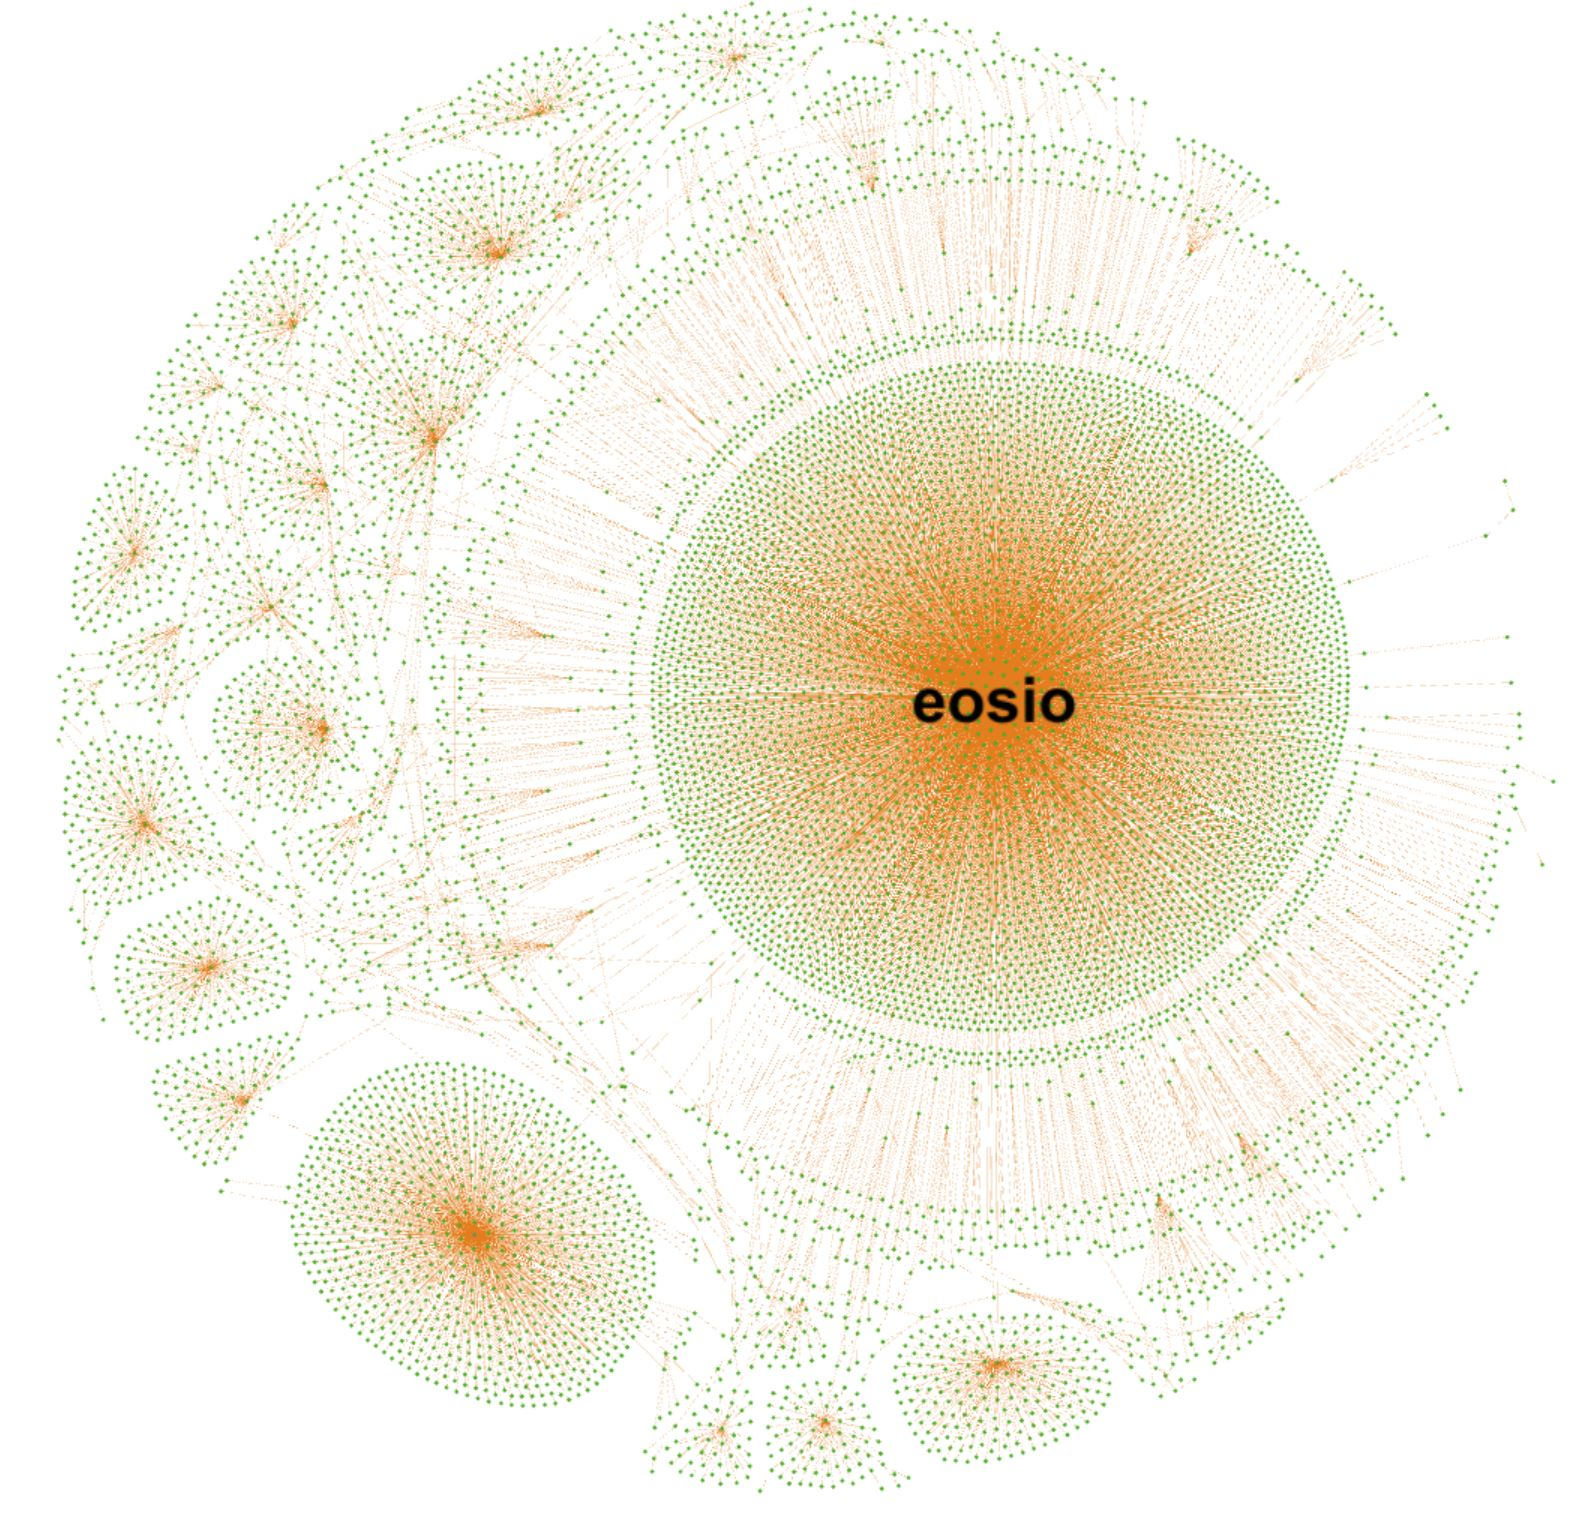
\includegraphics[scale=0.05, trim = 100 0 100 0]{figures/user_visual.jpg}
    }
    \subfigure[AVG]{%
    \label{fig:AVGVisualization}
    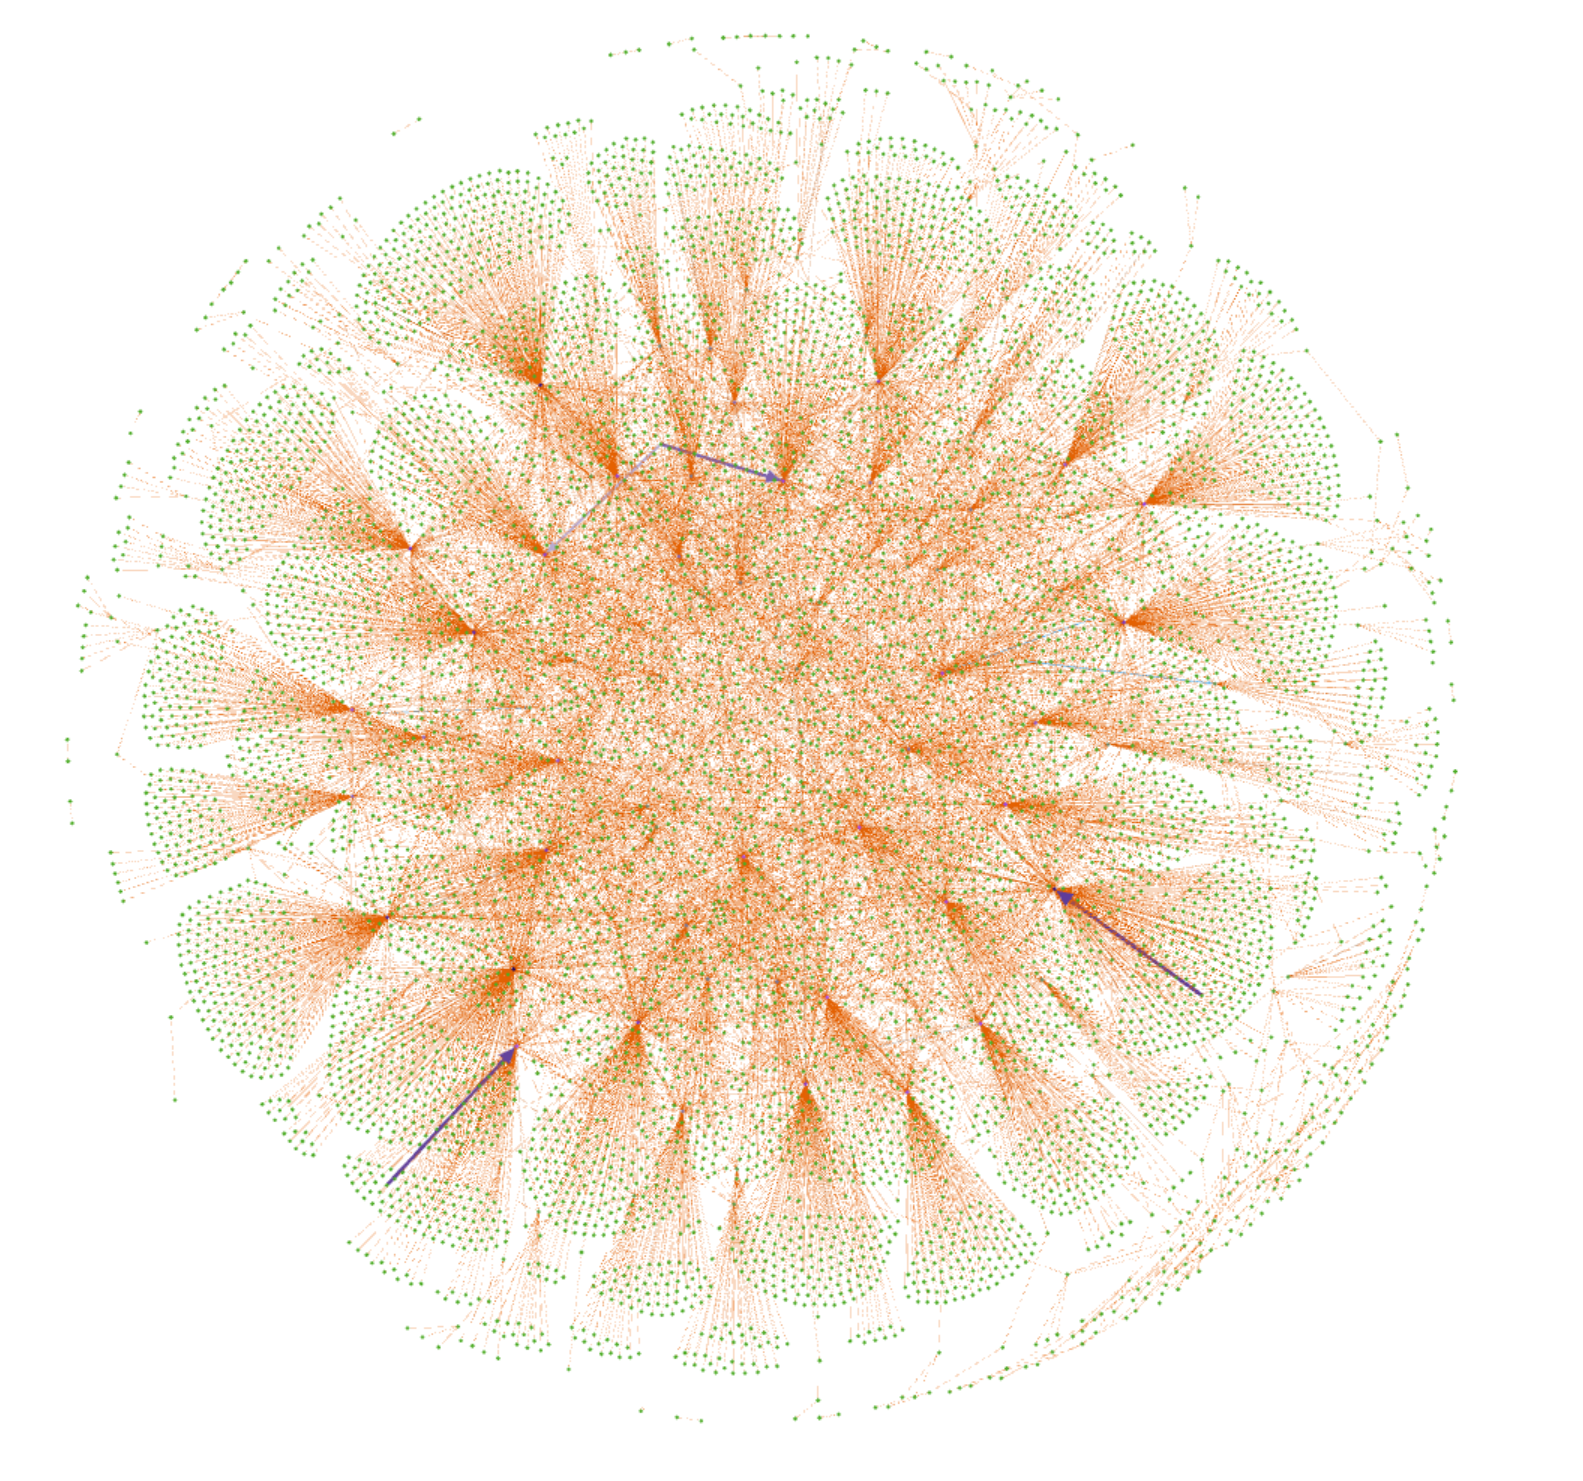
\includegraphics[scale=0.06, trim = 100 0 100 0]{figures/vote_visual.jpg}
    }
    \subfigure[MTG]{%
    \label{fig:MTGVisualization}
    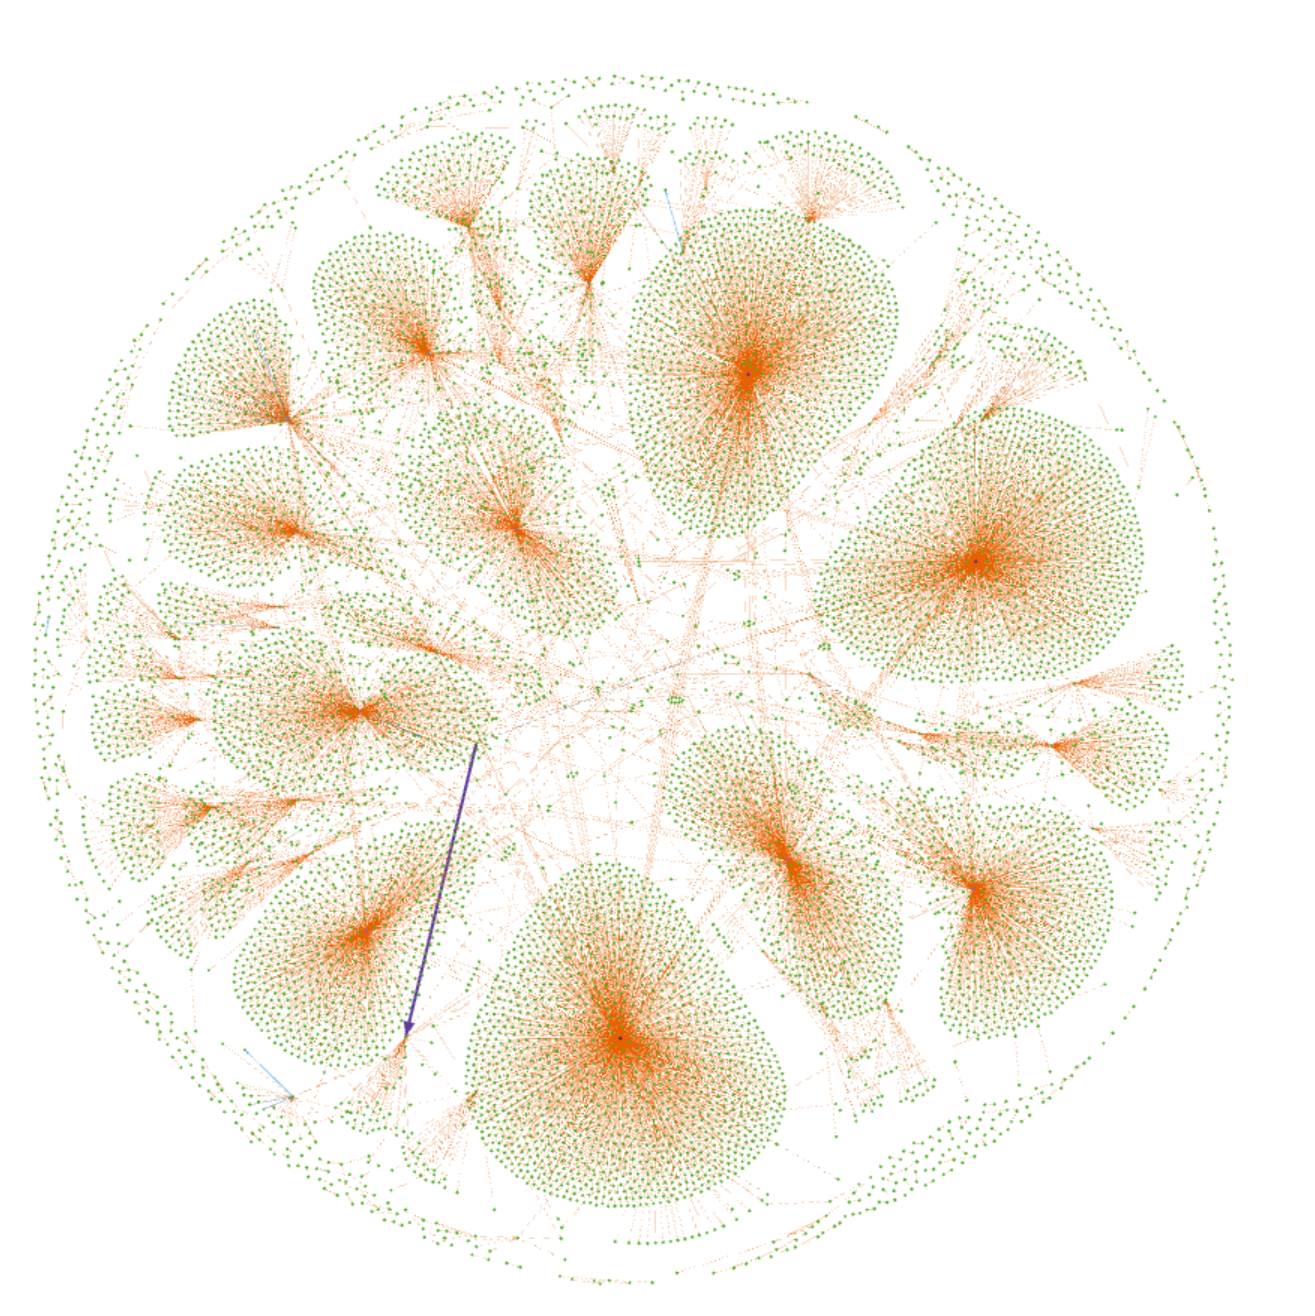
\includegraphics[scale=0.065, trim = 100 0 100 0]{figures/tx_visual.jpg}
    }
    \subfigure[CAG]{%
    \label{fig:CAGVisualization}
    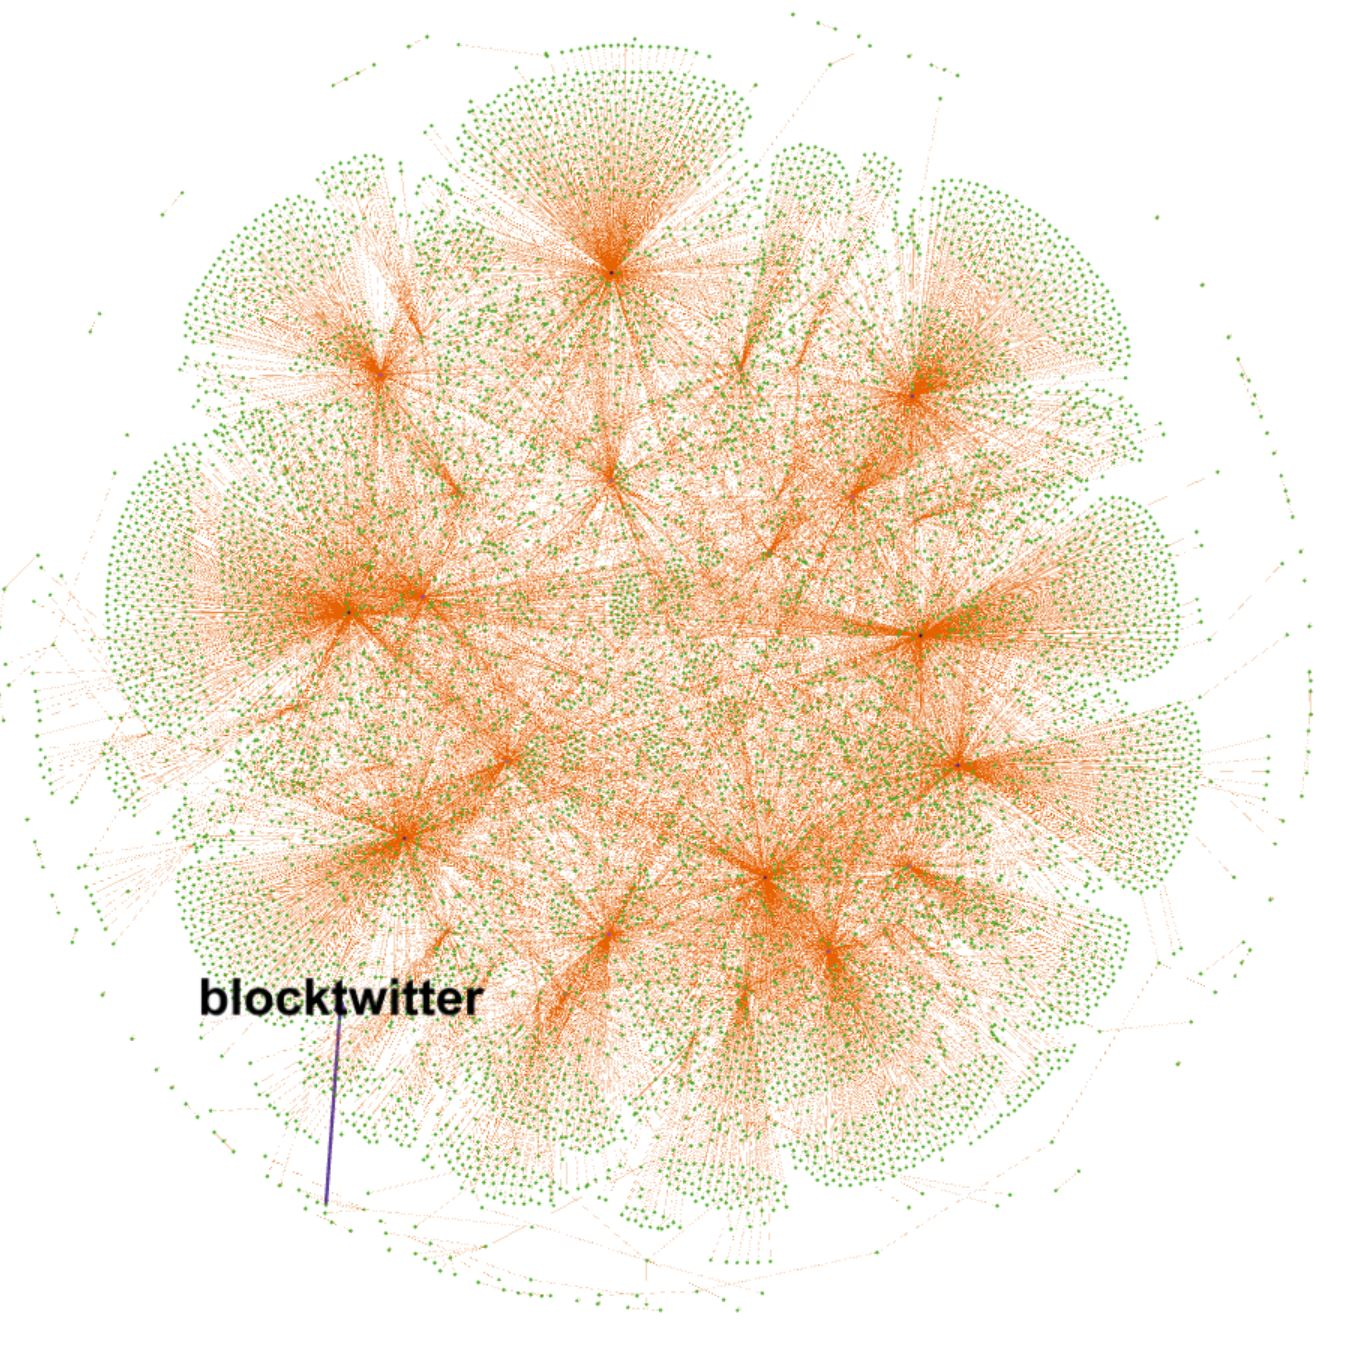
\includegraphics[scale=0.05, trim = 100 0 100 0]{figures/con_visual.jpg}
    }
    %
\centering
\label{fig:Visualization}
\end{figure}

\begin{table}
\centering
\caption{Statistic of Graphs}
\begin{tabular}{|c|c|c|}
     \hline
     \centering
     Graph & edges & nodes \\
     \hline
     ACG & 302,038 & 302,039 \\
     \hline
     AVG & 439,154 & 28,769 \\
     \hline
     MTG & 1,370,813 & 204,841 \\
     \hline
     CAG & 126,918 & 35,479 \\
     \hline
\end{tabular}
\label{Table:Statistic}
\end{table}

\subsection{Accounts creation}
\begin{figure}[htbp]
\centering
    \subfigure[ degree]{%
    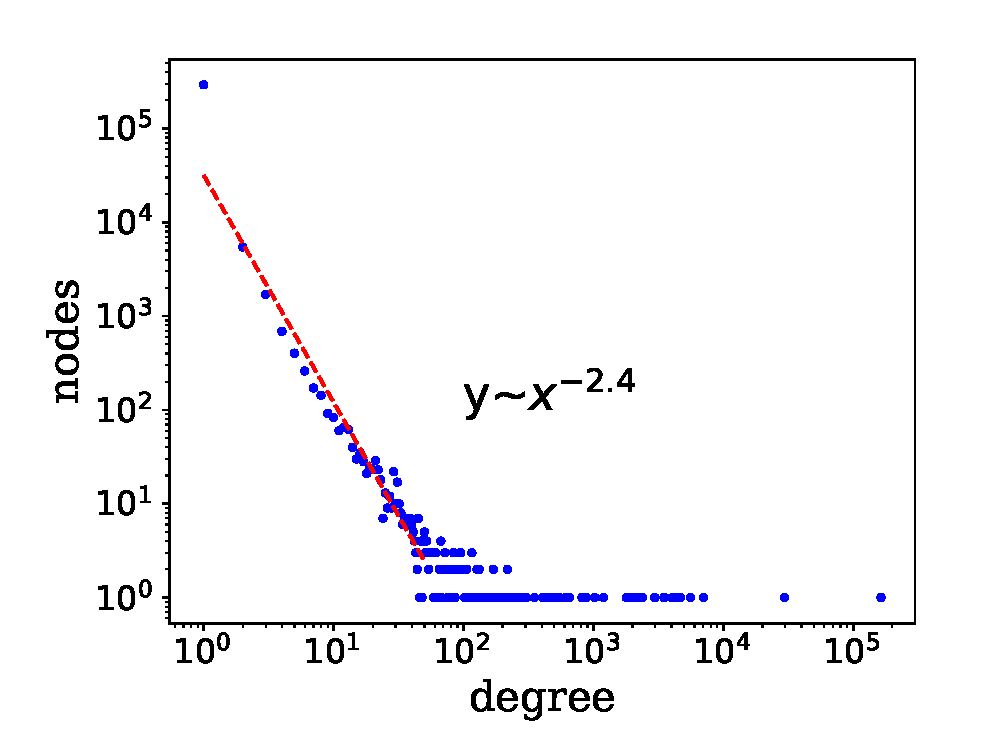
\includegraphics[scale=0.3]{figures/user_degree.eps}
    }
    \subfigure[ outdegree]{%
    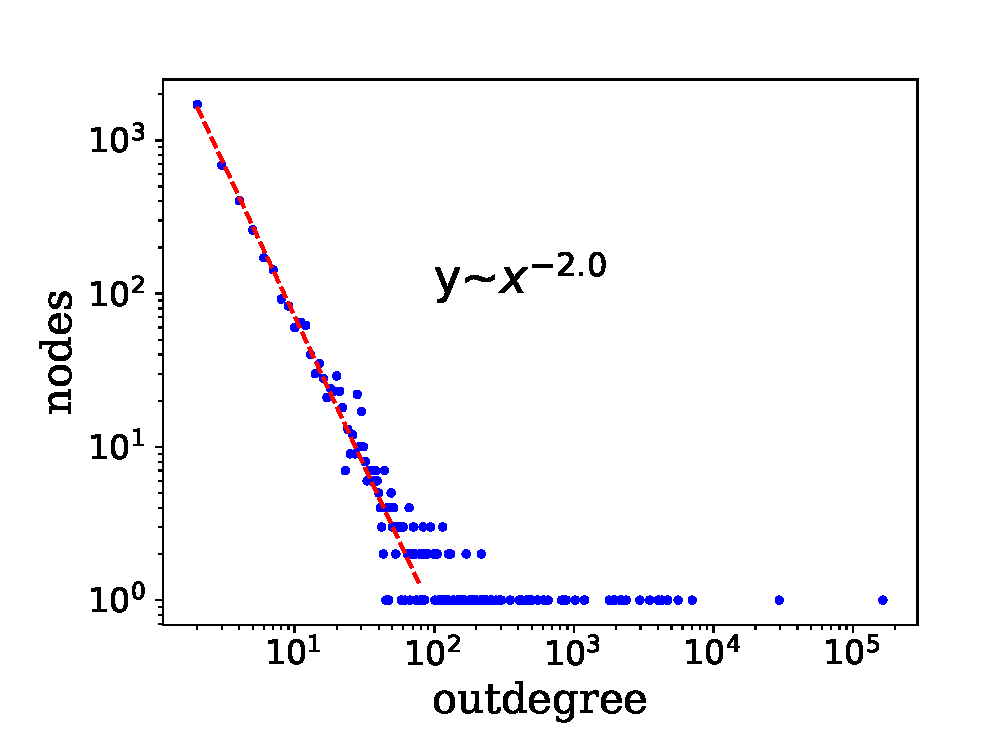
\includegraphics[scale=0.3]{figures/user_outdegree.eps}
    }
    %
\centering
\caption{ Degree/Indegree/Outdegree distributins of ACG}
\label{fig:ACGdegree}
\end{figure}

\begin{table}
 \caption{table:Metrics of Graphs}
 \begin{tabular}{|c|c|c|c|c|c|c|c|c|}
     \hline
     \centering
     Graph & Cluster & Assortativity & SCC & largest  SCC & WCC & largest WCC & largest diameter &  smallest diameter \\
     \hline
     ACG & 0 & / & 302,039 & 1 & 1 & 302,039 & 20 & 20 \\
     \hline
     AVG & 0.066 & -0.221 & 28,750 & 1 & 3 & 28,766 & 6 & 1 \\
     \hline
     MTG & 0.259 & -0.338 & 149,536 & 1 & 1 & 204,841 & 6 &  6 \\
     \hline
     CAG & 0.086 & -0.16 & 35,462 & 1 & 223 & 35,086 & 10 & 0\\
     \hline
\end{tabular}
\label{table:Metrics of Graphs}
\end{table}
New accounts can be created by old ones during account creation activities. To model this fact, we define ACG as follows:

$G=\{E,V\},\;\ E=\{v_i,v_j\},\;\ v_i,v_j\in V$,

where $V$ is a set of nodes, which represents accounts. $E$ is a set of edges, in which each pair of them represents the creation relationship.

The definition of ACG implies several properties. First of all, if $(v_i,v_j)\in E$, $k\ne i$, then $(v_k,v_j)\notin E$. Because one account only can be created by one father account, there is only one directed edge between two accounts. Secondly,  if $(v_i,v_j)\in E$,  then $(v_j,v_i)\notin E$. It implies that creating two accounts by each other is impossible.


We visualize ACG, as Figure. \ref{fig:ACGVisualization} shows. In this figure, we apply Union-Find algorithm to randomly select 8000 nodes and its pioneer nodes to guarantee every node to have a path to its ancestor node. There are several amazing observations. The whole graph is a tree-like graph, and every node has a directed path to eosio. In addition, most of them have one degree, namely they do not have child nodes. This may be because accounts are created by official accounts firstly, and then these created accounts can create others. So the root node of ACG is the official account eosio, while other accounts are directly or indirectly connecting with it in an unidirectional path. Therefore, we can see that the largest subgraph is the graph itself. Moreover, as Table \ref{Table:Statistic} shows, the number of edges is the same as that of actions, meaning one account cannot be created twice. In addition, the phenomenon that node number is one less than edge number also indicates the tree-like structure of ACG.

The outdegree and degree distributions of ACG satisfy power law distribution and have a long trailing, which are shown in Fig. \ref{fig:ACGdegree}. These distributions indicate that a few accounts have a large degree, creating many accounts. Besides, since the eosio have no indegree, and others have one for they only can be created once, the indegree of ACG is either 0 or 1, so we do not analyze the indegree of ACG.

We compute graph metrics of ACG and present them in Table. \ref{table:Metrics of Graphs}, such as the values of clustering  coefficient, assortativity coefficient, number of SCC/WCC, size (how many nodes) of largest SCC/WCC and largest/smallest diameter. The clustering coefficient is 0, since any accounts created by the same accounts cannot create each other. The largest diameter 20 is equal to the smallest one, indicating that the height of the tree-like graph is 20 and the only subgraph in ACG is the graph itself.

The largest SCC has one node, since every node can only be created once. The largest WCC have 302039 nodes, equal to all of nodes the whole ACG have, meaning that ACG is a WCC, because two accounts cannot be created each other, as well as the whole graph is a tree with the root of eosio.


\subsection{AVG Analysis}
\begin{figure}[htbp]
\centering
    \subfigure[ degree]{%
    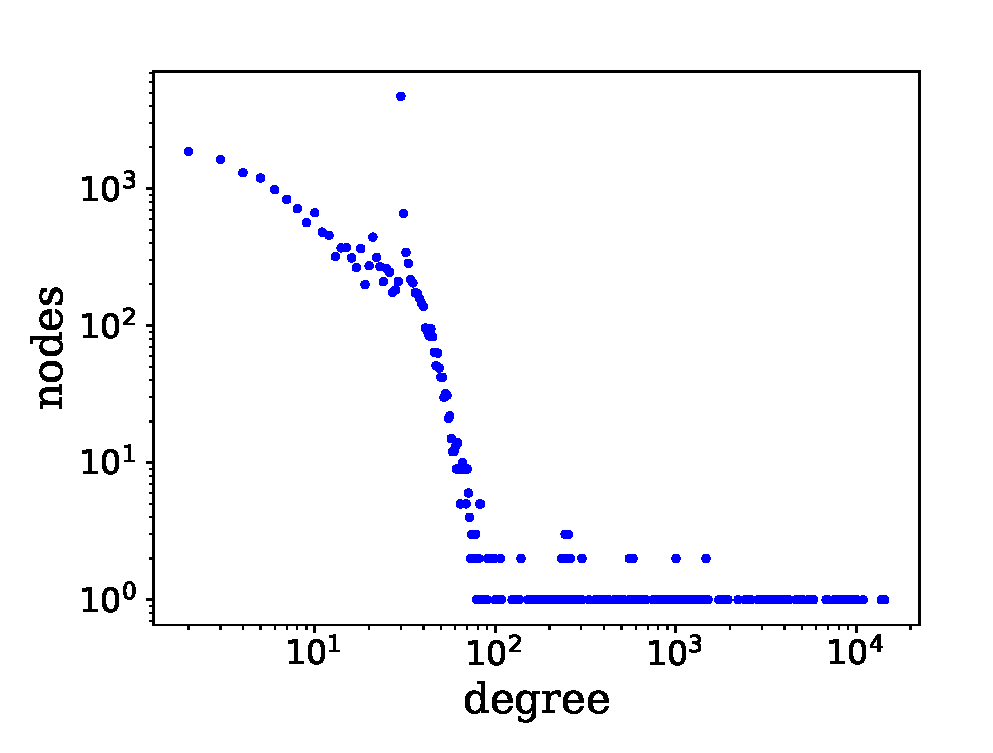
\includegraphics[scale=0.3]{figures/vote_degree.eps}
    }
    \subfigure[ indegree]{%
    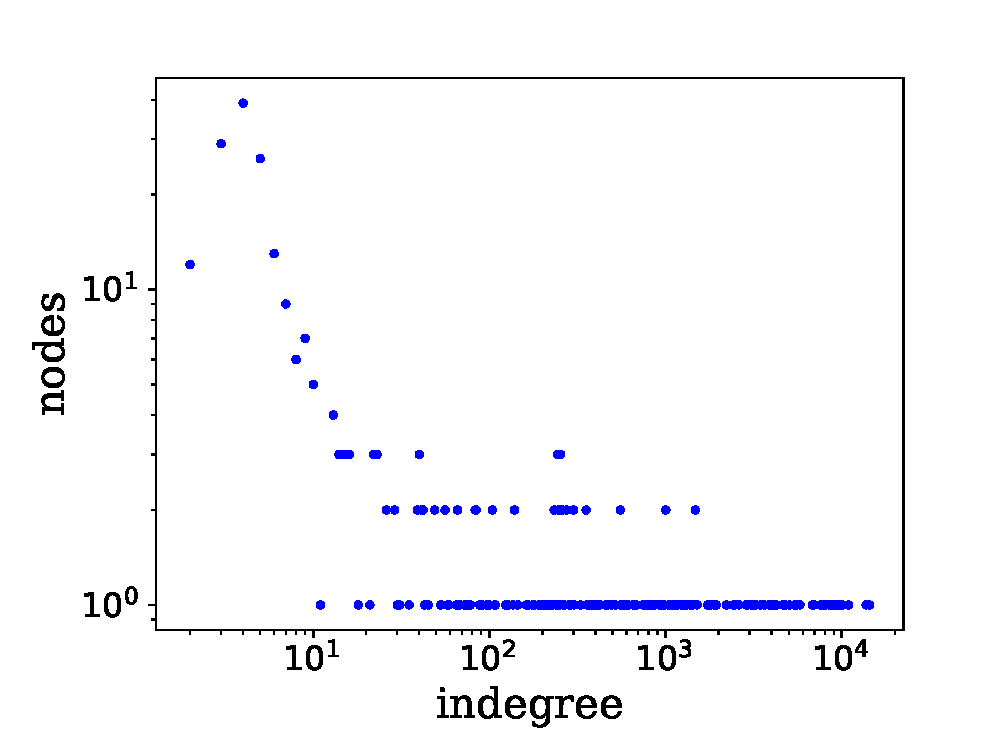
\includegraphics[scale=0.3]{figures/vote_indegree.eps}
    }
    \subfigure[ outdegree]{%
    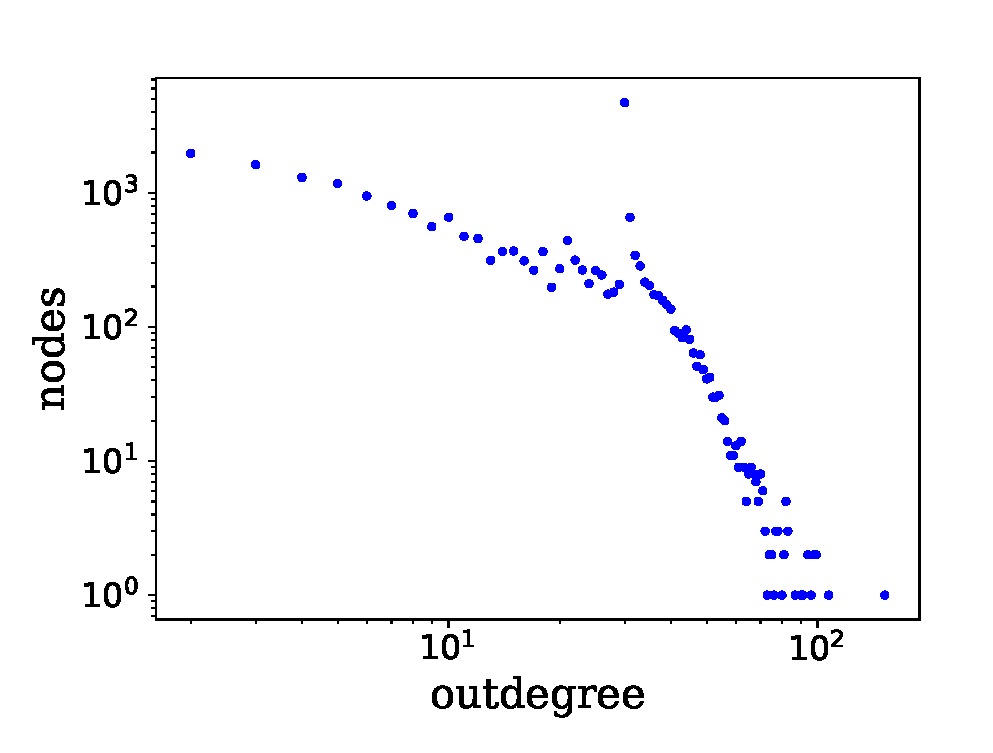
\includegraphics[scale=0.3]{figures/vote_outdegree.eps}
    }
    %
\centering
\caption{ Degree/Indegree/Outdegree distributins of AVG}
\label{fig:AVGdegree}
\end{figure}
Accounts can vote for others so that we can construct a graph to handle vote relationship among accounts. The definition is as follows:

$G=\{E,V,w\},\;\ E=\{v_i,v_j\},\;\ v_i,v_j\ \in\ V$,

where $V$ is a set of nodes, indicating accounts. $E$ is a set of edges, containing many ordered pairs of nodes, and each of them indicates a voter and a producer. $w$ refers to the total amounts of vote between certain pairs of nodes.

To visualize AVG, we randomly select 10000 edges. As we can see in Fig. \ref{fig:ACGVisualization}, most nodes in AVG have one degree. There are few accounts explicitly orientated to vote for others. The possible reason is that in the early period after the launch of mainnet, many voters were aimed to test EOSIO, or only wanted to experience voting, so the votes from them were greatly uncertain. Moreover, every account can vote for others, yet a few influential accounts can be voted by others. Thus, the graph is star-like, with many hub nodes who are respected producers. The statistics of AVG (Table. \ref{Table:Statistic}) demonstrate that there is a large gap between the number of actions and that of edges, suggesting that some voters often vote for one producers repeatedly. One possible conjecture is that those votes are used as part of a straw vote. But this is arguably not true because of the internal fairness of EOSIO. But it is more likely because some producers are very capable so that other accounts acknowledge it and are willing to vote for it. In addition, the total nodes who participate in voting only account for 9.5\% of all the accounts on EOSIO, which shows an appearance of false prosperity.

As shown in Fig. \ref{fig:AVGdegree}, the degree/ indegree/ outdegree distributions of AVG do not match power law distribution. We inspect these distributions. Many accounts vote for others only once, and few nodes vote many times. Moreover, the indegree distribution is the same as degree distribution, which suggesting that most accounts are voter, not producer. So in EOSIO, all accounts can be voters, while a few of them can be producers.

Table. \ref{table:Metrics of Graphs} lists the metrics of AVG. The clustering coefficient is 0.066, i.e. the percentage of tuples among accounts existing in AVG is low. Assortativity coefficient is negative, which can be explained that the nodes with many votes tend to vote for those with few votes whose competitiveness is far lower than the former ones. The largest diameter is 6 means that at most 6 accounts vote for others one by one. The small clustering and the small diameter illustrate that AVG is not a small world network.

The largest SCC have one node, revealing that two accounts are unlikely to vote for each other. Surprisingly, the largest WCC have 28,766 nodes, accounting for 93.4\% of AVG, which is large and covers almost the whole graph. The number of SCC is large, so WCC contains many SCCs, which means that only few votes concentrate in the small scales, while most votes are spread around the WCC.

\subsection{Money transfers}
\begin{figure}[htbp]
\centering
    \subfigure[ degree]{%
    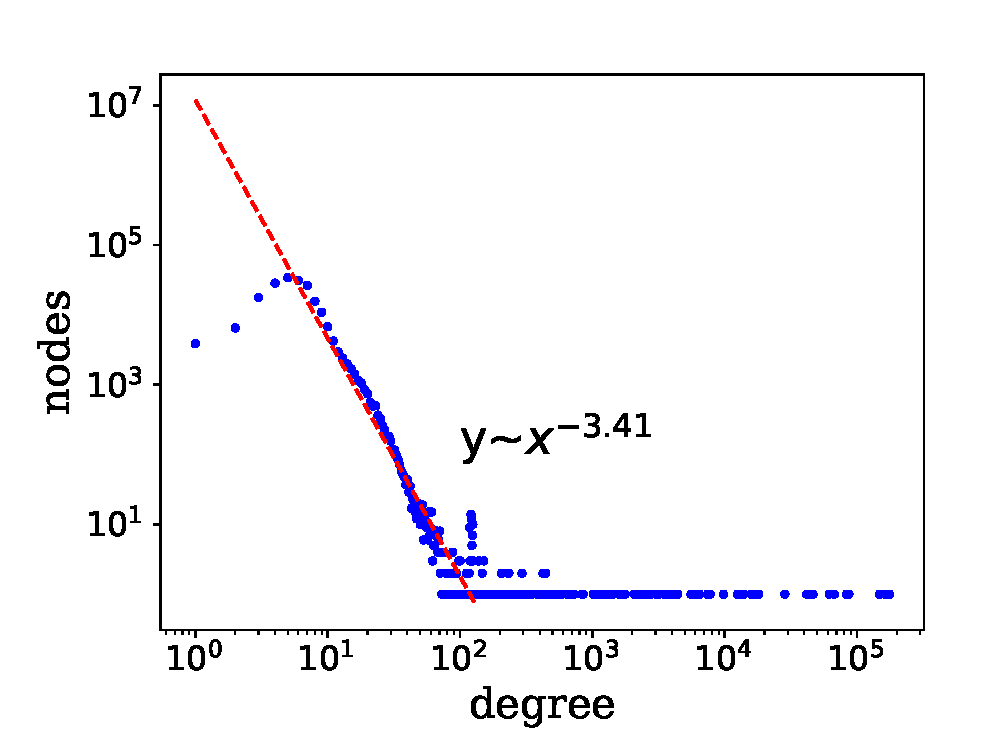
\includegraphics[scale=0.3]{figures/tx_degree.eps}
    }
    \subfigure[indegree]{%
    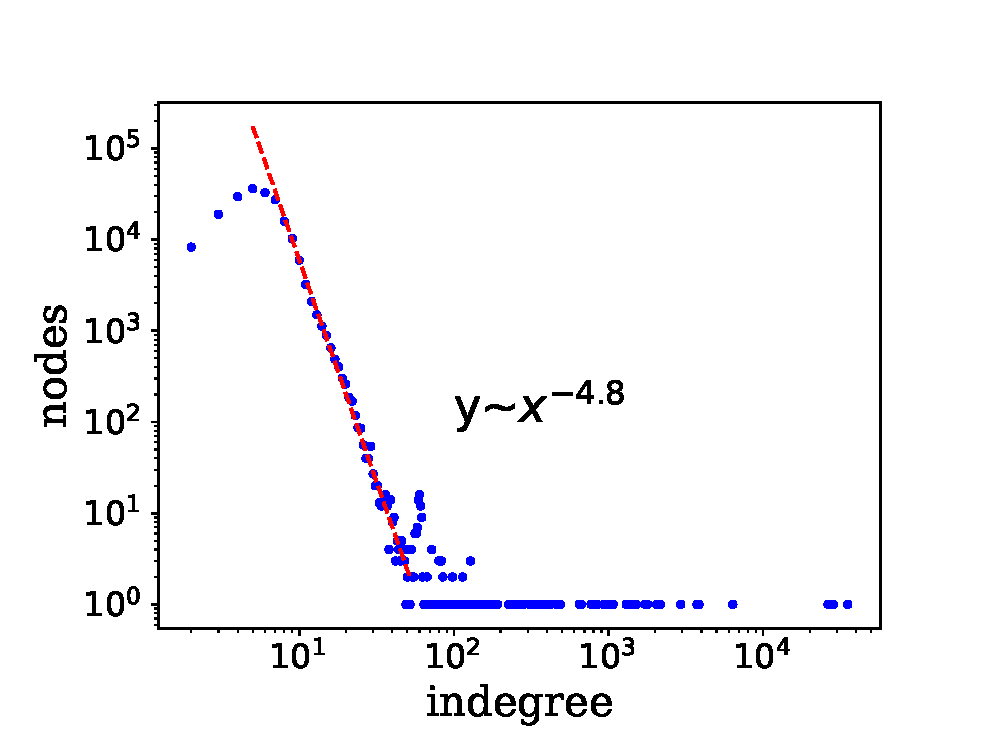
\includegraphics[scale=0.3]{figures/tx_indegree.eps}
    }
    \subfigure[outdegree]{%
    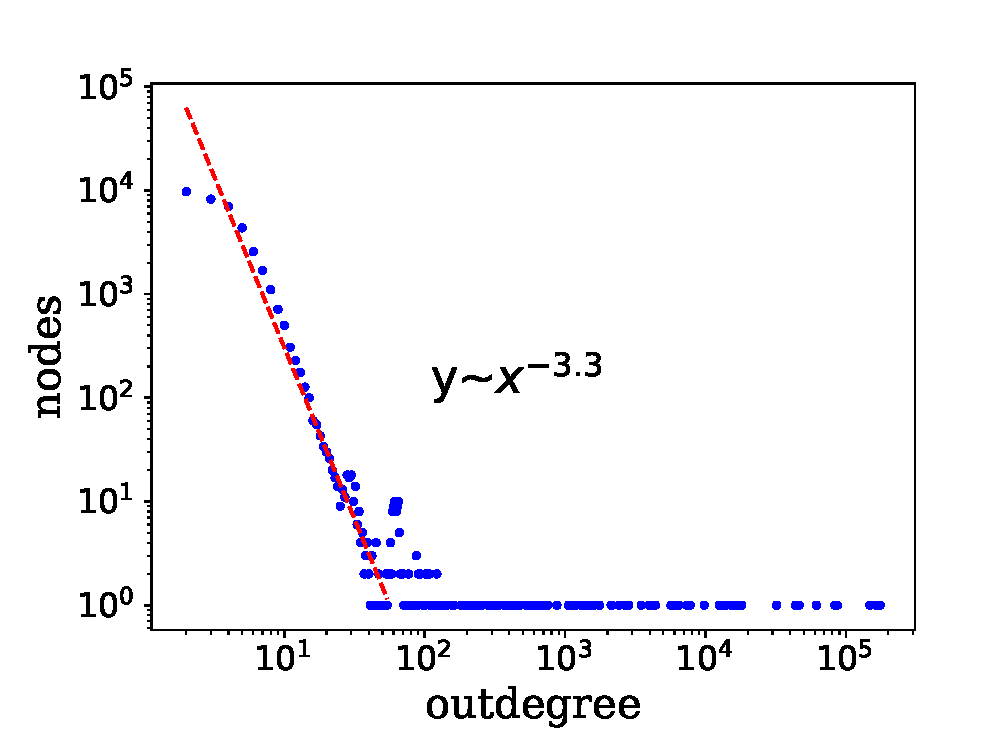
\includegraphics[scale=0.3]{figures/tx_outdegree.eps}
    }
    %
\centering
\caption{ Degree/Indegree/Outdegree distributins of MTG}
\label{fig:MTGGdegree}
\end{figure}
We construct a graph that indicates the transfer relationship among accounts. The definition is as follows:

$ G=\{E,V,w\},\;\ E={v_i,v_j},\;\ v_i,v_j\in V$,

where $V$ is a set of nodes, indicating accounts. $E$ is a set of edges, consisting of lots of ordered pairs of nodes, which indicates the direction of money transfer. $w$ refers to the total from a sender to a recipient.

MTG is visualized in Fig. \ref{fig:MTGVisualization}, where we randomly choose 10000 edges. A few large degree nodes (possibly are DApps and exchanges) and many small degree nodes (the individual users) constitute MTG. In particular, the fact that individual users can transfer money with others directly illustrates the free usage of EOSIO, which is unbelievable for former blockchain platform. Table. \ref{Table:Proportion} shows the statistic of MTG. As for the transfer action number is triple of the edges, we can obtain when one node want transfer to another, it will divide the money values into several times. The total accounts are only 67\% of all accounts on EOSIO, which means EOSIO is a platform with an illusion of prosperity.

The degree/ indegree/ outdegree distributions of MTG are shown in Table. \ref{Table:Statistic}, all of which are followed by the power law, meaning that a few large-degree nodes trade many times, while many small-degree nodes only trade once. The fitting line we plot on the figure shows coefficient $\alpha$ of the distribution $y~x^\alpha$. The larger $\alpha$ is, the more quickly the degree distribution varies. We inspect the fitting lines and  that indegree is more variable than degree/outdegree, which means one-degree recipients are far more than one-degree senders. These one-degree nodes probably are EOSIO fans or experiencers.

Table. \ref{Table:Proportion} shows some metrics of MTG. The clustering coefficient is 0.259, which is a moderately large value, indicating that when one account transfer to other two accounts respectively, these two accounts will have a transfer relationship. This tuple structure actually ensures the stable of the whole graph. Assortativity coefficient is negative, revealing an account with many trades prefers to transfer to accounts with few trades, and this matches the observation of visualization that DAPPs and exchanges who domain EOSIO are likely to trade with individuals.

The largest SCC have only one node, illustrating that there is no accounts trading with each other, since the aim of transfer is not to take back the money. Also, EOSIO is inherently a fair ecosystem, because accounts allocate resource (RAM, CPU, and NET) according to the number of tokens they hold, which means if you do not have enough money, you cannot attack others, but if you attack the system holding lots of tokens, it will cause a bad environment for your own trades. Thus, it is not surprising that there is few accounts can disturb the order of EOSIO community by ��scalping��. Moreover, the number of one-node SCCs is 149536, which is much more than the number of WCCs. It suggests that one WCC contains many one-node SCCs. The only WCC in MTG may be because the official account eosio transfer to many other accounts during mainnet launch, while these accounts almost have no transfer to each other. Consequently, the WCC is potentially supported by eosio account.

\subsection{Contracts authorization}
\begin{figure}[htbp]

\centering
    \subfigure[ degree]{%
    \includegraphics[scale=0.3]{figures/contract����degree.eps}
    }
    \subfigure[outdegree]{%
    \includegraphics[scale=0.3]{figures/contract����outdegree.eps}
    }
    \subfigure[ indegree]{%
    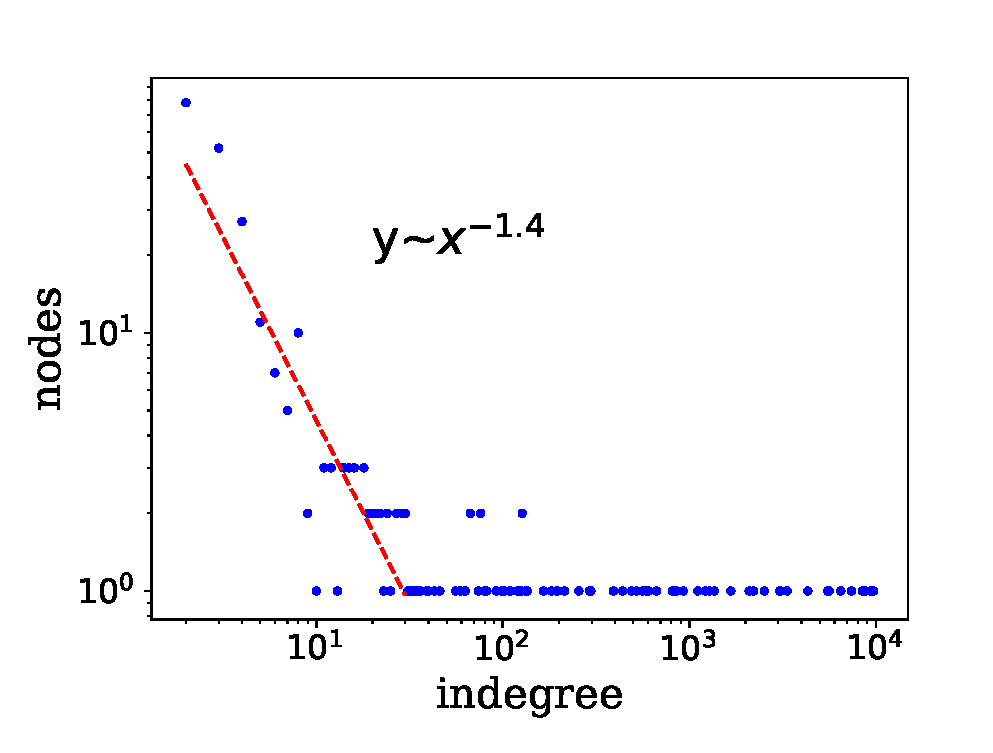
\includegraphics[scale=0.3]{figures/contract_indegree.eps}
    }
    %
\centering
\caption{ Degree/Indegree/Outdegree distributins of CAG}
\label{fig:CAGdegree}
\end{figure}
Contracts can authorize permissions to provide others access to execute actions. We construct CAG to describe this management relationship. The definition is shown as follows:

$G=\{E,V,w\},\;\ E=\{v_i,v_j\},\;\ v_i,v_j \in V$,

where $V$ is a set of nodes, which indicates contracts. $E$ is a set of edges, representing an authority between ordered pair of nodes. $w$ refers to the total times of authorizations between a certain pair of nodes.

To visualize CAG in Fig.\ref{fig:ACGVisualization}, we randomly choose 10000 edges. This indicates the existence of a few contract with large managing authority, and that those contracts defend their authority by managing the permissions of action such as transfer and vote.From the large gap between number of actions and edges (Table.  \ref{Table:Statistic}), we can see that some contracts are authorized many times. We inspect the data and find that in the total 331,530,705 edges, there are 316,579,248 edges authorized to one contracts named 'blocktwitter'. Although these authority have no real meaning, they cause the resource crisis of EOSIO, which impedes money transfer of others. In a word, 'blocktwitter�� is classed as a Denial of Service attack contact.

\ref{fig:CAGdegree} shows the degree/ indegree/ outdegree distributions of CAG. All the distributions meet power law distribution, namely, there are few nodes are authorized for many times, yet most nodes are authorized only once (possibly are DAPPs), which indicates that EOSIO are dominated by some influential DAPPs.

As \ref{table:Metrics of Graphs} shown, clustering coefficient is 0.086, which is not large, suggesting that when one contract authorizes other two contracts, the authority relationship between these two authorized contracts is unlikely to exist. Assortavity coefficient is negative, illustrating that the contracts with many permissions prefer to authorize those with few permissions, which seems to be a positive pyramid management structure. The smallest diameter is 0, meaning that there are contracts authorize themselves the permission to their actions. The largest diameter is 10, which shows that it is a large graph, and that many contracts authorize each other and maintain the operation of EOSIO by deploying various commercial applications.

The largest SCC is a one-node graph, manifesting that if one contract authorizes another one, it will have no authority of the previously authorized one. However, we do not exclude the phenomenon that accounts have its own authority. The largest WCC have 35086 nodes, which accounts for 90\% of CAG. But there are only 2 WCCs with more than 100 nodes, demonstrating that except the largest one, almost all WCCs are small.
